%%%%%%%%%%%%%%%%%%%%%%%%%%%%%%%%%%%%%%%%%
% University/School Laboratory Report
% LaTeX Template
% Version 4.0 (March 21, 2022)
%
% This template originates from:
% https://www.LaTeXTemplates.com
%
% Authors:
% Vel (vel@latextemplates.com)
% Linux and Unix Users Group at Virginia Tech Wiki
%
% License:
% CC BY-NC-SA 4.0 (https://creativecommons.org/licenses/by-nc-sa/4.0/)
%
%%%%%%%%%%%%%%%%%%%%%%%%%%%%%%%%%%%%%%%%%

%----------------------------------------------------------------------------------------
%	PACKAGES AND DOCUMENT CONFIGURATIONS
%----------------------------------------------------------------------------------------

\documentclass[
	letterpaper, % Paper size, specify a4paper (A4) or letterpaper (US letter)
	10pt, % Default font size, specify 10pt, 11pt or 12pt
]{CSUniSchoolLabReport}

%----------------------------------------------------------------------------------------
%	REPORT INFORMATION
%----------------------------------------------------------------------------------------

\title{ECE 398-MA \\ Introduction to Modern Communication with Python and SDR \\ Lab 8 -- FSK} % Report title

\author{Noah Breit} % Author name(s), add additional authors like: '\& James \textsc{Smith}'

\date{\today} % Date of the report

%----------------------------------------------------------------------------------------

\begin{document}

\maketitle % Insert the title, author and date using the information specified above

% \begin{center}
% 	\begin{tabular}{l r}
% 		Date Performed: & February 13, 2022 \\ % Date the experiment was performed
% 		Partners: & Cecilia \textsc{Smith} \\ % Partner names
% 		& Tajel \textsc{Khumalo} \\
% 		Instructor: & Professor \textsc{Rivera} % Instructor/supervisor
% 	\end{tabular}
% \end{center}

% If you need to include an abstract, uncomment the lines below
%\begin{abstract}
%	Abstract text
%\end{abstract}

%----------------------------------------------------------------------------------------
%	OBJECTIVE
%----------------------------------------------------------------------------------------

\section{Assignment 1}

\begin{lstlisting}[language=Python]
	import matplotlib.pyplot as plt
	import numpy as np
	from scipy.signal import resample_poly, butter, filtfilt, find_peaks
	
	
	def rrcosfilter(N, alpha, Tb, Fs):
	"""
	Generates a root raised cosine (RRC) filter (FIR) impulse response.
	
	Parameters
	----------
	N : int
	Length of the filter in samples.
	
	alpha : float
	Roll off factor (Valid values are [0, 1]).
	
	Tb : float
	Symbol period.
	
	Fs : float
	Sampling Rate.
	
	Returns
	---------
	h_rrc : 1-D ndarray of floats
	Impulse response of the root raised cosine filter.
	"""
	
	T_delta = 1/float(Fs)
	sample_num = np.arange(N)
	h_rrc = np.zeros(N, dtype=float)
	
	for x in sample_num:
	t = (x-N/2)*T_delta
	if t == 0.0:
	h_rrc[x] = 1.0 - alpha + (4*alpha/np.pi)
	elif alpha != 0 and t == Tb/(4*alpha):
	h_rrc[x] = (alpha/np.sqrt(2))*(((1+2/np.pi)* (np.sin(np.pi/(4*alpha)))) + ((1-2/np.pi)*(np.cos(np.pi/(4*alpha)))))
	elif alpha != 0 and t == -Tb/(4*alpha):
	h_rrc[x] = (alpha/np.sqrt(2))*(((1+2/np.pi)* (np.sin(np.pi/(4*alpha)))) + ((1-2/np.pi)*(np.cos(np.pi/(4*alpha)))))
	else:
	h_rrc[x] = (np.sin(np.pi*t*(1-alpha)/Tb) +
	4*alpha*(t/Tb)*np.cos(np.pi*t*(1+alpha)/Tb))/ (np.pi*t*(1-(4*alpha*t/Tb)*(4*alpha*t/Tb))/Tb)
	
	return h_rrc
	
	
	
	# Create random binary data and BPSK symbols from the previous labs
	num_data_symbols = 32
	sps = 16
	Tb = 1
	
	np.random.seed(0)
	bits = np.random.randint(0, 2, num_data_symbols) # 0 to 1
	bpsk_symbols = bits*2 - 1
	############ YOUR CODE STARTS HERE ############
	barker = np.array([1,1,1,1,1,-1,-1,1,1,-1,1,-1,1])
	# Concatenate TWO sets of Barkers, guard interval, and data to create a frame here
	guard = np.zeros_like(barker) 
	frame = np.concatenate((barker, barker, guard, bpsk_symbols))
	# Upsample and perform pulse-shaping here (the pulse is given)
	up_sym = np.zeros(len(frame)*sps)
	up_sym[::sps] = frame  # Symbol-spaced upsampling
	# Tx_ADC is the pulse-shaped signal
	
	num_taps = 6*sps + 1
	pulse = rrcosfilter(N=num_taps, alpha=1.0, Tb=sps, Fs=1)
	Tx_ADC = np.convolve(up_sym, pulse)
	Tx_ADC = np.concatenate((np.zeros(sps*10), Tx_ADC)) # pad more zeros to help frame sync simulation
	
	############ YOUR CODE ENDS HERE ############  
	
	############################################
	## Simulate IQ modulator (Tx)
	############################################
	M = 16  # upsample fs_adc for pass-band simulation
	xup = resample_poly(Tx_ADC, M, 1)
	fs_adc = sps    # sampling rate of ADC
	fs_rf = M * fs_adc  # sampling rate for simulating carrier
	fc = (M*3/7) * fs_adc # carrier frequency
	t = 1/fs_rf*np.arange(len(xup)) # time vector at fs_rf
	
	# u(t): transmitted signal to the channel (passband)
	u = np.real(xup) * np.cos(2*np.pi*fc*t) - np.imag(xup) * np.sin(2*np.pi*fc*t)
	############################################
	## Simulate Channel
	############################################
	ch_att = 0.1    # channel attenuation
	
	h = np.zeros(M*sps)
	h[0] = ch_att
	h = np.roll(h, np.random.randint(M*sps))    # random delay
	
	v = np.convolve(u, h) 
	noise_amplitude = 0.01
	noise = noise_amplitude * np.random.randn(len(v))   # AWGN
	
	v = v + noise
	############################################
	## Simulate IQ demodulator (Rx)
	############################################
	# Low-Pass Filter (LPF) @ fc
	Nfilt = 5
	cutoff = fc
	b, a = butter(Nfilt, Wn=cutoff, btype='low', fs=fs_rf)
	t = 1/fs_rf*np.arange(len(v))
	
	# Add CFO
	N = len(barker)
	cfo_limit = 1/(2*N*Tb)
	# cfo_hz = cfo_limit*0.05
	# cfo_hz = -cfo_limit*0.05
	cfo_hz = cfo_limit*1.05
	print('CFO limit (Hz): +- ', cfo_limit)
	print('Applied CFO (Hz): ', cfo_hz)
	
	yI = filtfilt(b, a, v*np.cos(2*np.pi*(fc + cfo_hz)*t))
	yQ = filtfilt(b, a, -v*np.sin(2*np.pi*(fc + cfo_hz)*t))
	
	Rx_ADC = resample_poly(yI + 1j*yQ, 1, M)
	############ YOUR CODE STARTS HERE ############
	# Matched filtering and symbol timing recovery from the previous labs here
	rx_matched = np.convolve(Rx_ADC, pulse)
	
	# Compute energy for each alignment offset
	energy = np.zeros(sps)
	for k in range(sps):
	# Compute energy for each offset by summing squared values of sampled segments
	energy[k] = np.sum(np.abs(rx_matched[k::sps])**2)
	
	# Find the best offset
	max_ind = np.argmax(energy)
	print("max_ind: ", max_ind)
	
	# Align samples using max_ind
	rx_aligned = rx_matched[max_ind::sps]
	
	# Self-reference Frame synchronization: compute N-lagged auto-correlation (corr) and detect the peak (frame_ind)
	N = len(barker)
	corr = np.zeros(len(rx_aligned) - 2*N)
	for n in range(len(corr)):
	sum = 0
	for k in range(N):
	sum += np.conj(rx_aligned[n+k]) * rx_aligned[n+k+N]
	corr[n] = np.abs(sum) / N
	
	frame_ind = np.argmax(corr)
	
	# Plot the correlation and its peak
	plt.figure
	plt.plot(corr)
	plt.plot(frame_ind, corr[frame_ind], 'x', label=f'frame_ind={frame_ind}')
	plt.title('self-reference correlation')
	plt.grid(True)
	plt.legend()
	# plt.savefig('assignment1a.png')
	# plt.savefig('assignment1d.png')
	plt.savefig('assignment1g.png')
	plt.show()
	
	# Plot the received data and frame start
	# plt.figure
	# plt.plot(rx_aligned)
	# plt.plot(frame_ind, rx_aligned[frame_ind], 'x', label=f'frame_ind={frame_ind}')
	# plt.title('demodulated rx signal')
	# plt.grid(True)
	# plt.legend()
	# plt.show()
	
	# Separate preamble and data symbols
	rx_preamble = rx_aligned[frame_ind:frame_ind+2*N]
	rx_data = rx_aligned[frame_ind+3*N:frame_ind+3*N+num_data_symbols]
	
	#################################
	# Estimate CFO_
	#################################
	
	# Calculate delta_phi
	products = np.conj(rx_preamble[:N]) * rx_preamble[N:2*N]
	sum_product = np.sum(products) / len(products)
	delta_phi = np.angle(sum_product)
	
	cfo_hat = delta_phi / (2*np.pi*N*Tb)
	
	# Compare the estimation with the ground truth
	print("cfo_hz: ", cfo_hz)
	# print("cfo_hat: ", cfo_hat)
	print("cfo_hat: ", cfo_hat)
	
	#################################
	# Correct CFO_
	#################################
	t_cfo = np.arange(len(rx_aligned)) * Tb
	rx_cfo_corrected = rx_aligned * np.exp(-1j*2*np.pi*cfo_hat*t_cfo)
	rx_preamble_CFOcor = rx_cfo_corrected[frame_ind:frame_ind+2*N]
	rx_data_CFOcor = rx_cfo_corrected[frame_ind+3*N:frame_ind+3*N+num_data_symbols]
	
	############ YOUR CODE ENDS HERE ############
	# Create the IQ constellation_
	plt.figure
	plt.subplot(1,2,1)
	plt.plot(rx_preamble.real, rx_preamble.imag, '.')
	plt.xlabel('I')
	plt.ylabel('Q')
	plt.title('Preamble sym Before CFO corr')
	plt.grid(True)
	plt.xlim([-1.2, 1.2])
	plt.ylim([-1.2, 1.2])
	ax = plt.gca()
	ax.set_aspect('equal', adjustable='box')
	plt.subplot(1,2,2)
	plt.plot(rx_data.real, rx_data.imag, '.')
	plt.xlabel('I')
	plt.ylabel('Q')
	plt.title('Data sym Before CFO corr')
	plt.grid(True)
	plt.xlim([-1.2, 1.2])
	plt.ylim([-1.2, 1.2])
	ax = plt.gca()
	ax.set_aspect('equal', adjustable='box')
	# plt.savefig('assignment1b.png')
	# plt.savefig('assignment1e.png')
	plt.savefig('assignment1h.png')
	plt.show()
	
	# Create the IQ constellation_
	plt.figure
	plt.subplot(1,2,1)
	plt.plot(rx_preamble_CFOcor.real, rx_preamble_CFOcor.imag, '.')
	plt.xlabel('I')
	plt.ylabel('Q')
	plt.title('Preamble sym After CFO corr')
	plt.grid(True)
	plt.xlim([-1.2, 1.2])
	plt.ylim([-1.2, 1.2])
	ax = plt.gca()
	ax.set_aspect('equal', adjustable='box')
	plt.subplot(1,2,2)
	plt.plot(rx_data_CFOcor.real, rx_data_CFOcor.imag, '.')
	plt.xlabel('I')
	plt.ylabel('Q')
	plt.title('Data sym After CFO corr')
	plt.grid(True)
	plt.xlim([-1.2, 1.2])
	plt.ylim([-1.2, 1.2])
	ax = plt.gca()
	ax.set_aspect('equal', adjustable='box')
	# plt.savefig('assignment1c.png')
	# plt.savefig('assignment1f.png')
	plt.savefig('assignment1i.png')
	plt.show()
\end{lstlisting}

\begin{figure}[H] % [H] forces the figure to be placed exactly where it appears in the text
	\centering % Horizontally center the figure
	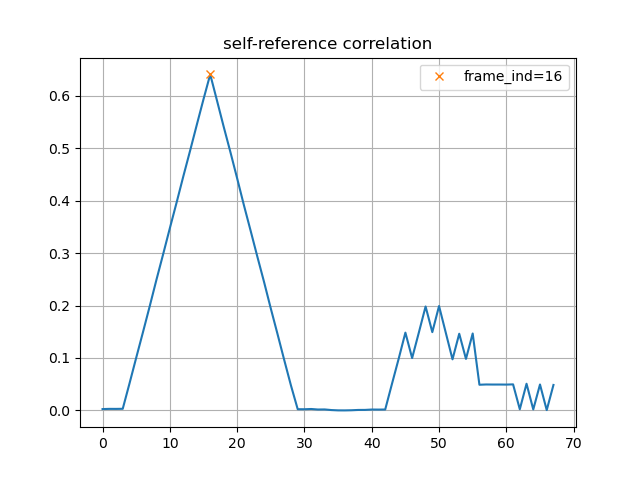
\includegraphics[width=1.2\textwidth]{assignment1a.png} % Include the figure
	\caption{self-reference corr: cfo\_hz = cfo\_limit*0.05}
	\label{fig:block}
\end{figure}
SERIAL-OUT self-reference corr: cfo\_hz = cfo\_limit*0.05\newline
CFO\ limit (Hz): +-  0.038461538461538464\newline
Applied CFO (Hz):  0.0019230769230769232\newline
max\_ind:  8\newline
cfo\_hz:  0.0019230769230769232\newline
cfo\_hat:  0.001987514744180262\newline

\begin{figure}[H] % [H] forces the figure to be placed exactly where it appears in the text
	\centering % Horizontally center the figure
	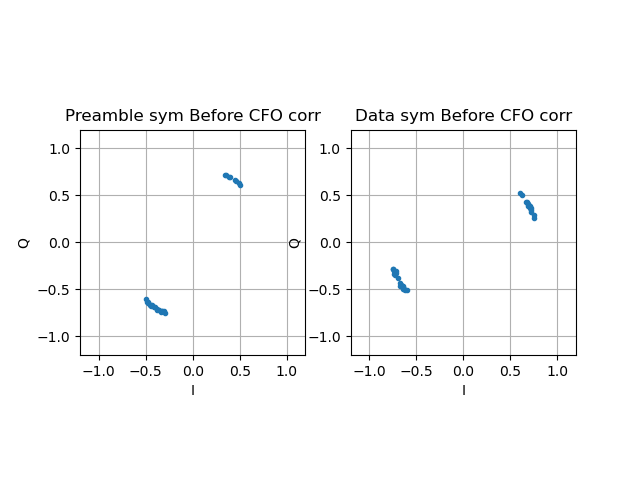
\includegraphics[width=1.2\textwidth]{assignment1b.png} % Include the figure
	\caption{Preamble IQ Plot: cfo\_hz = cfo\_limit*0.05}
	\label{fig:block}
\end{figure}

\begin{figure}[H] % [H] forces the figure to be placed exactly where it appears in the text
	\centering % Horizontally center the figure
	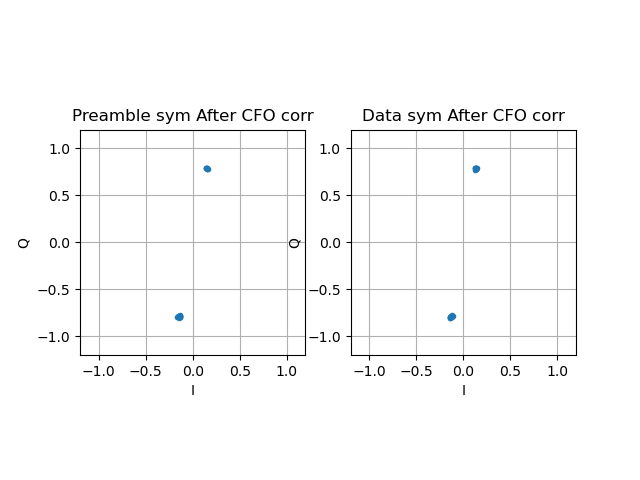
\includegraphics[width=1.2\textwidth]{assignment1c.png} % Include the figure
	\caption{Data Symbols IQ Plot: cfo\_hz = cfo\_limit*0.05}
	\label{fig:block}
\end{figure}

\begin{figure}[H] % [H] forces the figure to be placed exactly where it appears in the text
	\centering % Horizontally center the figure
	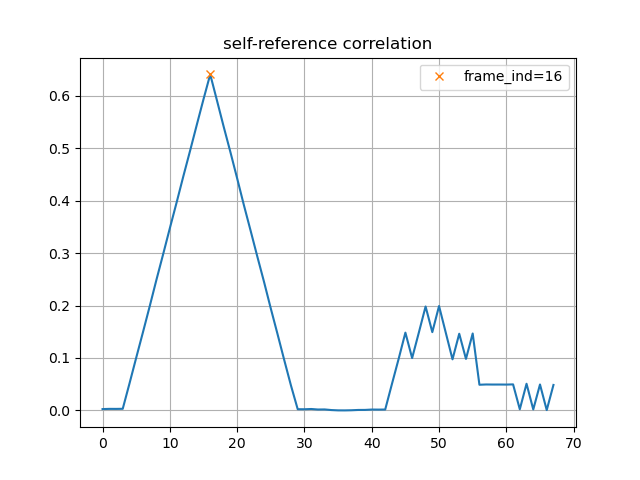
\includegraphics[width=1.2\textwidth]{assignment1d.png} % Include the figure
	\caption{self-reference corr: cfo\_hz = -cfo\_limit*0.05}
	\label{fig:block}
\end{figure}
SERIAL-OUT self-reference corr: cfo\_hz = -cfo\_limit*0.05\newline
CFO limit (Hz): +-  0.038461538461538464\newline
Applied CFO (Hz):  -0.0019230769230769232\newline
max\_ind:  8\newline
cfo\_hz:  -0.0019230769230769232\newline
cfo\_hat:  -0.001858604409919798\newline

\begin{figure}[H] % [H] forces the figure to be placed exactly where it appears in the text
	\centering % Horizontally center the figure
	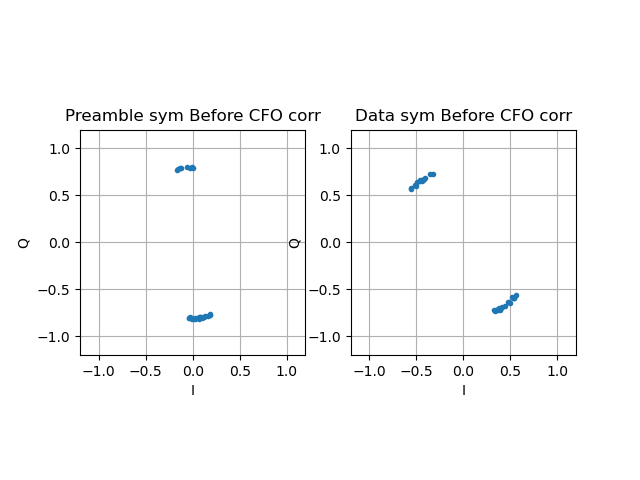
\includegraphics[width=1.2\textwidth]{assignment1e.png} % Include the figure
	\caption{Preamble IQ Plot: cfo\_hz = -cfo\_limit*0.05}
	\label{fig:block}
\end{figure}

\begin{figure}[H] % [H] forces the figure to be placed exactly where it appears in the text
	\centering % Horizontally center the figure
	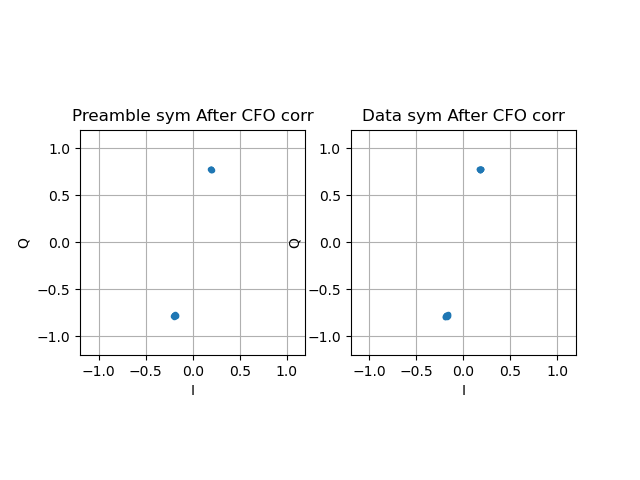
\includegraphics[width=1.2\textwidth]{assignment1f.png} % Include the figure
	\caption{Data Symbols IQ Plot: -cfo\_hz = cfo\_limit*0.05}
	\label{fig:block}
\end{figure}

\begin{figure}[H] % [H] forces the figure to be placed exactly where it appears in the text
	\centering % Horizontally center the figure
	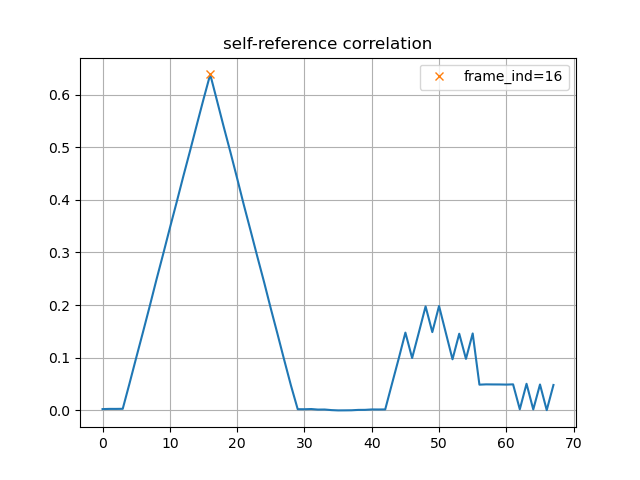
\includegraphics[width=1.2\textwidth]{assignment1g.png} % Include the figure
	\caption{self-reference corr: cfo\_hz = cfo\_limit*1.05}
	\label{fig:block}
\end{figure}
SERIAL-OUT self-reference corr: cfo\_hz = cfo\_limit*1.05\newline
CFO limit (Hz): +-  0.038461538461538464\newline
Applied CFO (Hz):  0.04038461538461539\newline
max\_ind:  8\newline
cfo\_hz:  0.04038461538461539\newline
cfo\_hat:  -0.036474784731455996\newline

<clearly failed!!>this CFO correction failed because the channel error causes data to perform a full rotation around the polar axis.

\begin{figure}[H] % [H] forces the figure to be placed exactly where it appears in the text
	\centering % Horizontally center the figure
	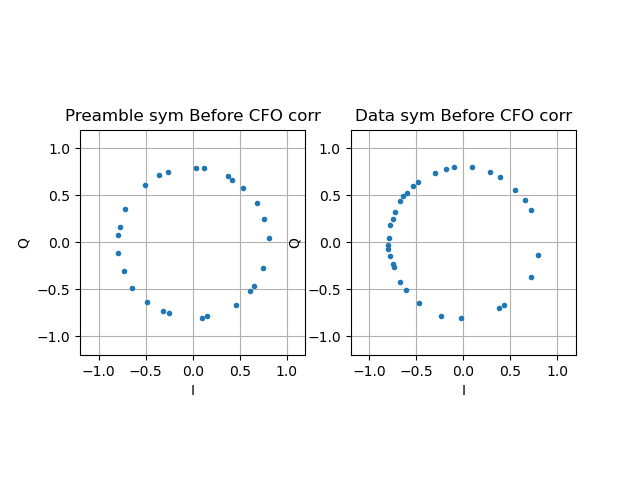
\includegraphics[width=1.2\textwidth]{assignment1h.png} % Include the figure
	\caption{Preamble IQ Plot: cfo\_hz = cfo\_limit*1.05}
	\label{fig:block}
\end{figure}

\begin{figure}[H] % [H] forces the figure to be placed exactly where it appears in the text
	\centering % Horizontally center the figure
	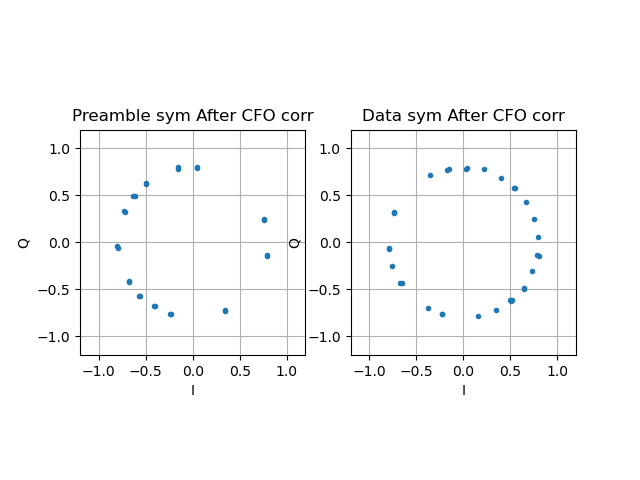
\includegraphics[width=1.2\textwidth]{assignment1i.png} % Include the figure
	\caption{Data Symbols IQ Plot: cfo\_hz = cfo\_limit*1.05}
	\label{fig:block}
\end{figure}

\begin{lstlisting}[language=Python]
	############# ASSIGNMENT 2 ##############
	
	#################################
	# Estimate/Correct Channel_
	#################################
	barker2 = np.concatenate((barker, barker))
	
	h_hat = np.mean(rx_preamble_CFOcor / barker2)
	rx_preamble_CHcor = rx_preamble_CFOcor / h_hat
	rx_data_CHcor = rx_data_CFOcor / h_hat
	
	print("h_hat:", h_hat)
	
	# Create the IQ constellation_
	plt.figure
	plt.subplot(1,2,1)
	plt.plot(rx_preamble_CHcor.real, rx_preamble_CHcor.imag, '.')
	plt.xlabel('I')
	plt.ylabel('Q')
	plt.title('Preamble sym After CH corr')
	plt.grid(True)
	plt.xlim([-1.2, 1.2])
	plt.ylim([-1.2, 1.2])
	ax = plt.gca()
	ax.set_aspect('equal', adjustable='box')
	plt.subplot(1,2,2)
	plt.plot(rx_data_CHcor.real, rx_data_CHcor.imag, '.')
	plt.xlabel('I')
	plt.ylabel('Q')
	plt.title('Data sym After CH corr')
	plt.grid(True)
	plt.xlim([-1.2, 1.2])
	plt.ylim([-1.2, 1.2])
	ax = plt.gca()
	ax.set_aspect('equal', adjustable='box')
	# plt.savefig('assignment2a.png')
	# plt.savefig('assignment2b.png')
	plt.savefig('assignment2c.png')
	plt.show()
	
	#################################
	# Recover the bits_
	#################################
	rx_bits = np.zeros(len(rx_data_CHcor), dtype=int)
	for k in range(len(rx_data_CHcor)):
	if rx_data_CHcor[k].real > 0:  # BPSK
	rx_bits[k] = 1
	else:
	rx_bits[k] = 0
	
	# print("rx_data: ", rx_data)_
	print("original bits: ", bits)
	print("rx_bits: ", rx_bits)
	
	# bit error_
	bit_err = np.sum( np.abs(bits - rx_bits) )
	print("bit error: ", bit_err)
	print("bit error rate (%): ", 100*bit_err/num_data_symbols)
\end{lstlisting}

\begin{figure}[H] % [H] forces the figure to be placed exactly where it appears in the text
	\centering % Horizontally center the figure
	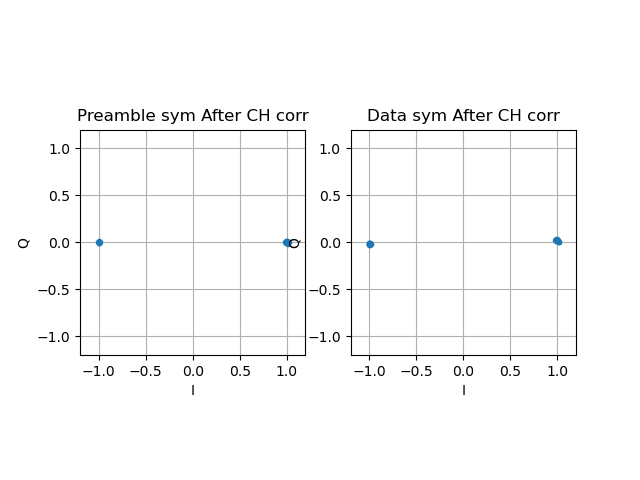
\includegraphics[width=1.2\textwidth]{assignment2a.png} % Include the figure
	\caption{self-reference corr: cfo\_hz = cfo\_limit*0.05}
	\label{fig:block}
\end{figure}

SERIAL-OUT self-reference corr: cfo\_hz = cfo\_limit*0.05\newline
CFO limit (Hz): +-  0.038461538461538464\newline
Applied CFO (Hz):  0.0019230769230769232\newline
max\_ind:  8\newline
cfo\_hz:  0.0019230769230769232\newline
cfo\_hat:  -0.001987514744180262\newline
h\_hat: (-0.1453780186634645-0.7872008939992515j)\newline
original bits:  [0 1 1 0 1 1 1 1 1 1 1 0 0 1 0 0 0 0 0 1 0 1 1 0 0 1 1 1 1 0 1 0]\newline
rx\_bits:  [0 1 1 0 1 1 1 1 1 1 1 0 0 1 0 0 0 0 0 1 0 1 1 0 0 1 1 1 1 0 1 0]\newline
bit error:  0\newline
bit error rate (%):  0.0\newline

\begin{figure}[H] % [H] forces the figure to be placed exactly where it appears in the text
	\centering % Horizontally center the figure
	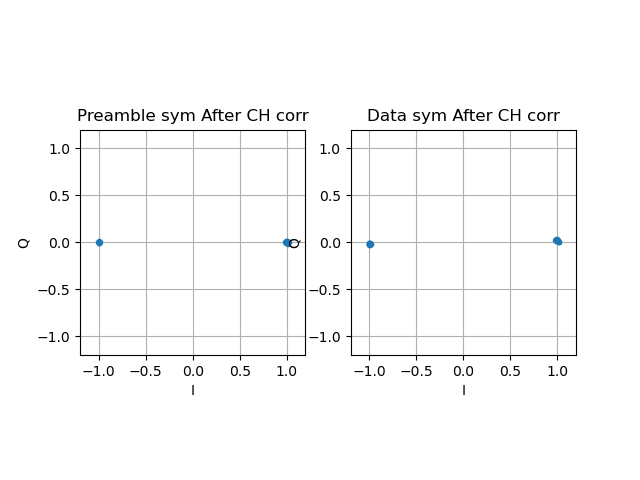
\includegraphics[width=1.2\textwidth]{assignment2b.png} % Include the figure
	\caption{self-reference corr: cfo\_hz = -cfo\_limit*0.05}
	\label{fig:block}
\end{figure}

SERIAL-OUT self-reference corr: cfo\_hz = -cfo\_limit*0.05\newline
CFO limit (Hz): +-  0.038461538461538464\newline
Applied CFO (Hz):  -0.0019230769230769232\newline
max\_ind:  8\newline
cfo\_hz:  -0.0019230769230769232\newline
cfo\_hat:  0.001858604409919798\newline
h\_hat: (-0.19312022183167252-0.776873416777837j)\newline
original bits:  [0 1 1 0 1 1 1 1 1 1 1 0 0 1 0 0 0 0 0 1 0 1 1 0 0 1 1 1 1 0 1 0]\newline
rx\_bits:  [0 1 1 0 1 1 1 1 1 1 1 0 0 1 0 0 0 0 0 1 0 1 1 0 0 1 1 1 1 0 1 0]\newline
bit error:  0\newline


\begin{figure}[H] % [H] forces the figure to be placed exactly where it appears in the text
	\centering % Horizontally center the figure
	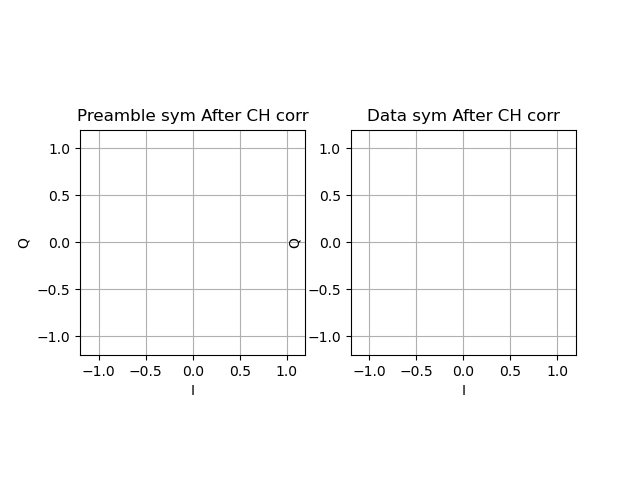
\includegraphics[width=1.2\textwidth]{assignment2c.png} % Include the figure
	\caption{self-reference corr: cfo\_hz = cfo\_limit*1.05}
	\label{fig:block}
\end{figure}

SERIAL-OUT self-reference corr: cfo\_hz = cfo\_limit*1.05\newline
CFO limit (Hz): +-  0.038461538461538464\newline
Applied CFO (Hz):  0.04038461538461539\newline
max\_ind:  8\newline
cfo\_hz:  0.04038461538461539\newline
cfo\_hat:  0.036474784731455996\newline
h\_hat: (0.00041507606418906146+0.0026299981006439386j)\newline
original bits:  [0 1 1 0 1 1 1 1 1 1 1 0 0 1 0 0 0 0 0 1 0 1 1 0 0 1 1 1 1 0 1 0]\newline
rx\_bits:  [1 0 1 0 1 1 1 1 0 0 0 1 1 0 1 0 0 0 0 1 0 0 0 1 1 0 0 0 1 0 1 0]\newline
bit error:  16\newline
bit error rate (%):  50.0\newline

\end{document}